\section{Referencia de la Clase Proveedor\-List}
\label{classProveedorList}\index{ProveedorList@{ProveedorList}}
Muestra y administra la ventana con el listado de proveedores.  


{\tt \#include $<$providerslist.h$>$}

Diagrama de colaboraci\'{o}n para Proveedor\-List:\begin{figure}[H]
\begin{center}
\leavevmode
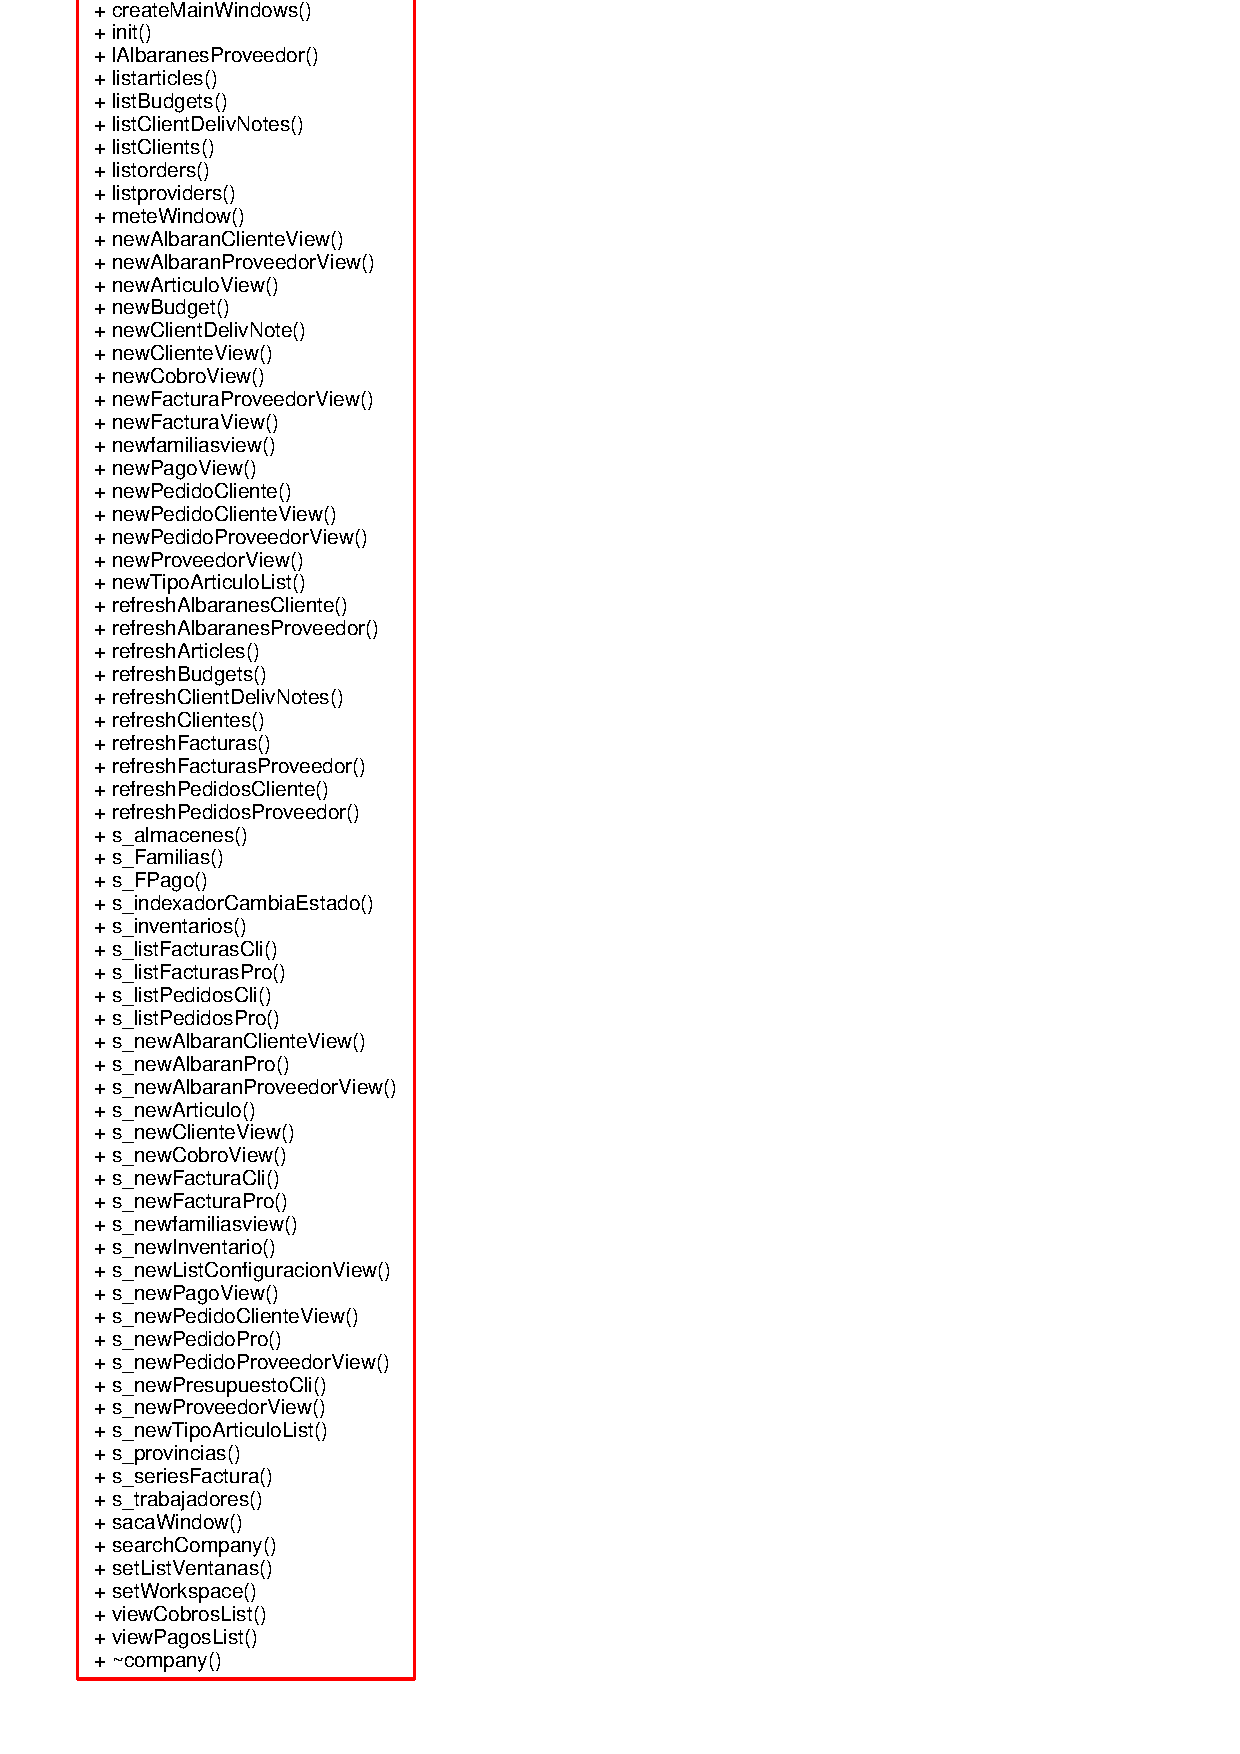
\includegraphics[width=119pt]{classProveedorList__coll__graph}
\end{center}
\end{figure}
\subsection*{Tipos p\'{u}blicos}
\begin{CompactItemize}
\item 
enum {\bf edmode} \{ {\bf Edit\-Mode} =  0, 
{\bf Select\-Mode} =  1
 \}
\end{CompactItemize}
\subsection*{Slots p\'{u}blicos}
\begin{CompactItemize}
\item 
virtual void {\bf editar} (int)\label{classProveedorList_i0}

\item 
virtual void {\bf on\_\-mui\_\-actualizar\_\-clicked} ()\label{classProveedorList_i1}

\item 
virtual void {\bf on\_\-mui\_\-borrar\_\-clicked} ()
\item 
virtual void {\bf on\_\-mui\_\-configurar\_\-toggled} (bool checked)\label{classProveedorList_i3}

\item 
virtual void {\bf on\_\-mui\_\-crear\_\-clicked} ()\label{classProveedorList_i4}

\item 
virtual void {\bf on\_\-mui\_\-editar\_\-clicked} ()\label{classProveedorList_i5}

\item 
virtual void {\bf on\_\-mui\_\-exportar\_\-clicked} ()\label{classProveedorList_i6}

\item 
virtual void {\bf on\_\-mui\_\-filtro\_\-text\-Changed} (const QString \&text)\label{classProveedorList_i7}

\item 
virtual void {\bf on\_\-mui\_\-importar\_\-clicked} ()\label{classProveedorList_i8}

\item 
virtual void {\bf on\_\-mui\_\-imprimir\_\-clicked} ()\label{classProveedorList_i9}

\begin{CompactList}\small\item\em SLOT que se ejecuta al pulsar sobre el boton de imprimir en la ventana de proveedores. \item\end{CompactList}\item 
void {\bf on\_\-mui\_\-list\_\-item\-Double\-Clicked} (QTable\-Widget\-Item $\ast$)\label{classProveedorList_i10}

\item 
virtual void {\bf s\_\-find\-Provider} ()\label{classProveedorList_i11}

\end{CompactItemize}
\subsection*{Se\~{n}ales}
\begin{CompactItemize}
\item 
void {\bf selected} (QString)\label{classProveedorList_l0}

\end{CompactItemize}
\subsection*{M\'{e}todos p\'{u}blicos}
\begin{CompactItemize}
\item 
QString {\bf cifprovider} ()\label{classProveedorList_a0}

\item 
void {\bf hide\-Botonera} ()\label{classProveedorList_a1}

\item 
void {\bf hide\-Busqueda} ()\label{classProveedorList_a2}

\item 
QString {\bf idprovider} ()\label{classProveedorList_a3}

\item 
void {\bf modoedicion} ()\label{classProveedorList_a4}

\item 
void {\bf modoseleccion} ()\label{classProveedorList_a5}

\item 
QString {\bf nomprovider} ()\label{classProveedorList_a6}

\item 
void {\bf presenta} ()\label{classProveedorList_a7}

\item 
{\bf Proveedor\-List} ({\bf company} $\ast$, QWidget $\ast$parent=0, Qt::WFlags flag=0, edmode editmode=Edit\-Mode)\label{classProveedorList_a8}

\item 
void {\bf show\-Botonera} ()\label{classProveedorList_a9}

\item 
void {\bf show\-Busqueda} ()\label{classProveedorList_a10}

\end{CompactItemize}


\subsection{Descripci\'{o}n detallada}
Muestra y administra la ventana con el listado de proveedores. 



\subsection{Documentaci\'{o}n de las funciones miembro}
\index{ProveedorList@{Proveedor\-List}!on_mui_borrar_clicked@{on\_\-mui\_\-borrar\_\-clicked}}
\index{on_mui_borrar_clicked@{on\_\-mui\_\-borrar\_\-clicked}!ProveedorList@{Proveedor\-List}}
\subsubsection{\setlength{\rightskip}{0pt plus 5cm}void Proveedor\-List::on\_\-mui\_\-borrar\_\-clicked ()\hspace{0.3cm}{\tt  [virtual, slot]}}\label{classProveedorList_i2}


SLOT que responde a la pulsacion de borrar un determinado proveedor Dicha funcion avisa de la perdida de datos y si se decide continuar Se procede a borrar el proveedor. 

La documentaci\'{o}n para esta clase fu\'{e} generada a partir de los siguientes archivos:\begin{CompactItemize}
\item 
providerslist.h\item 
providerslist.cpp\end{CompactItemize}
